%------------------------------ PREAMBLE. IKKE SÅ VIKTIG I FØRSTE OMGANG --------------------------------------------
\documentclass{article}     % Setter klassen til dokumentet
\usepackage[utf8]{inputenc}
\usepackage[norsk]{babel}
\usepackage{physics}
\usepackage{allrunes}
\usepackage{amsmath,amsfonts,amssymb,amsthm,mathtools} % Most people will need these for mathematics
\usepackage{color}
\usepackage[table]{xcolor}
\newcommand{\vect}[1]{\boldsymbol{#1}}
\usepackage[printwatermark]{xwatermark}
\usepackage{xcolor}
\usepackage{graphicx}
\usepackage{natbib}

%\newwatermark*[allpages,color=red!50,angle=45,scale=3,xpos=0,ypos=0]{UTKAST}



%Pakker for figurer
\usepackage{graphicx}	%Graphics package
%\usepackage[center]{caption}
\usepackage{subcaption}
\usepackage{wrapfig}  % Wrap text around figures
\usepackage{float} % To place figures correctly

\usepackage{makeidx} % Probably important.
\usepackage{listings}
\usepackage{color}
 
\definecolor{codegreen}{rgb}{0,0.6,0}
\definecolor{codegray}{rgb}{0.5,0.5,0.5}
\definecolor{codepurple}{rgb}{0.58,0,0.82}
\definecolor{backcolour}{rgb}{0.95,0.95,0.92}
 
\lstdefinestyle{mystyle}{
    backgroundcolor=\color{backcolour},   
    commentstyle=\color{codegreen},
    keywordstyle=\color{magenta},
    numberstyle=\tiny\color{codegray},
    stringstyle=\color{codepurple},
    basicstyle=\footnotesize,
    breakatwhitespace=false,         
    breaklines=true,                 
    captionpos=b,                    
    keepspaces=true,                 
    numbers=left,                    
    numbersep=5pt,                  
    showspaces=false,                
    showstringspaces=false,
    showtabs=false,                  
    tabsize=2
}
 
\lstset{style=mystyle}
\usepackage{color}
\usepackage{hyperref} % Clickable links to urls, internal and external references etc.
\usepackage{amsmath}
\usepackage[makeroom]{cancel}
\usepackage{siunitx}  %Write units easily \SI{value}

\lstset{
    basicstyle=\footnotesize\ttfamily,
  identifierstyle=\bfseries\color{green!40!black},
  commentstyle=\itshape\color{purple!40!black},
  keywordstyle=\color{blue},
  stringstyle=\color{orange},
}

\usepackage{pdfpages}	% Packages to handle certain issues with the pdf conversion and landscape figures/tables
\usepackage{lscape}

\usepackage[authoryear,square]{natbib} % References/bibliography package
\usepackage{footnote}
\usepackage{appendix} % Appendix + add to table of contents
\usepackage{sidecap}

% Table packages
\usepackage{tabularx}
\makesavenoteenv{tabular}
\makesavenoteenv{table}
\usepackage{array}
\usepackage{booktabs}
\newcommand*\rot{\rotatebox{90}}

%Special in-document vector graphics:
\usepackage{tikz}
\usetikzlibrary{shapes.geometric,calc,positioning,3d,intersections,arrows}
\usetikzlibrary{decorations.markings}
\usepackage{pgfplots}
\usepackage{circuitikz}  %Brukes til å enkelt tegne kretser

% Custom characters
\newcommand{\slfrac}[2]{\left.#1\middle/#2\right.} % Long on-line fraction-slash: \slfrac
\newcommand{\degree}{\ensuremath{^\circ}} % The 'degree' character : \degree
\DeclareRobustCommand{\orderof}{\ensuremath{\mathcal{O}}} % The 'Order of' character: \orderof




%------------------------------------------------- DOKUMENTET BEGYNNER HER ---------------------------------------------


%TITTEL. Her settes titellen til teksten.
\title{\vspace{-3.5cm}}
\title{
 \vspace{-3.5cm} Rapport INF-1400 \\ 
\begin{large} 
  Obligatorisk oppgave 1
\end{large} }

%FORFATTER. Her defineres forfatteren(e)
\author{%
	\large
	\textsc{Martin Soria Røvang}\\
	\normalsize	Universitetet i Troms{\o}
	\footnote{.} \\
	\vspace{-5mm}
	}


% START DOKUMENT
\begin{document}

\maketitle   % Skriver ut tittelen som ble definert ovenfor.

%ABSTRAKT/OPPSUMMERING

%Oppsummerer hele forsøket på en kort og konsis måte (100-300 ord).
%Førsteinntrykket!
%Følger gjerne samme oppsett som artikkelen:
%En setning om motivasjon/formål
%Kort beskrivelse metode
%Presenter resultater. Gi de viktigste tallene.
%Konklusjon

\section{Introduksjon}
I denne oppgaven skal man lage en klone av spillet $"$Breakout$"$ med mål om å bruke objektorientert design så godt som mulig. I denne rapporten blir det diskutert hvordan dette ble designet og implementert.

\subsection{Krav}
1. Implementer spillet etter objektorientert design, bruk objekter og klasser.\\
2. Platformen skal kunne kontrolleres med mus eller tastatur.\\
3. Ballen skal sprette i forskjellige retning basert på hvor på platformen den treffer.\\
4. En brikke skal forsvinne når ballen treffer den.\\
5. Spillet er vunnet når alle brikkene er fjernet, spillet er tapt hvis ballen går under skjermen ved platformen sin side.\\
6. Strukturert og kommentert kode.


\section{Teknisk bakgrunn}

\textbf{Pygame modul}: Pygame modul\footnote{https://www.pygame.org/wiki/GettingStarted} blir brukt for å tegne til skjermen. I dokumentasjonen til Pygame står det også om hvordan man initialiserer pygame vinduet som er nyttig for å komme igang.\\
\textbf{Attributter}: Attributter er egenskaper/verdier som ligger i klassen og/eller instansene som er laget fra klassene. Disse verdiene kan endres innad i hver enkelt instans.[\cite{Dustyphil} p.37]\\
\textbf{Klassemetoder}: Klasse-metodene er funksjoner som ligger inni instansene, slik at de kan bli kalt på direkte fra instansene. Disse funksjonene må ha med ett argument som normalt kalles \emph{self}. Denne gir deg mulighet til å hente ut metodene og attributtene fra klassen inn i denne spesifikke funksjonen. Hvis man legger med en @staticmethods over funksjonene gir man muligheten til å kalle på metoden fra klassen også(her vil man ikke få self argument).[\cite{Dustyphil} p.38]







\clearpage

%TEORI OG DEFINISJONER
%Presenter viktig teori for å kunne utføre og forstå eksperimentet.
%Hva tenger du/dine medstudenter å lære?

\section{Design}
\subsection{Klassestruktur}
I denne oppgaven har vi klassene som vist i figur(\ref{UML}) under,

\begin{figure}[h!]
\center{
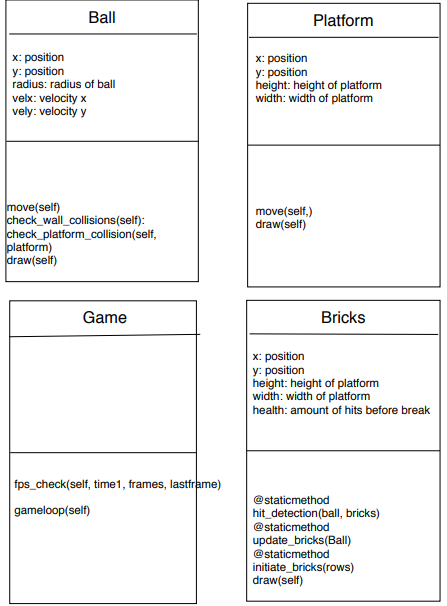
\includegraphics[width=0.70\textwidth]{UML.png}
}
\caption{UML diagram for alle klassene i prosjektet}
\label{UML}
\end{figure}

Her har vi brukt staticmethod på tre av metodene i $"$Bricks$"$ fordi \emph{hit\_detection}, \emph{update\_bricks} og \emph{initiate\_bricks} er bricks relevante metoder, men kjøres ikke direkte på objektene selv.
\subsection{Klassene}

Klasser fungerer som en blåkopi av et objekt man har lyst på. I denne blåkopien kan man fastsette \emph{attributtene} man vil at objektet skal starte med, dette gjøres ved spesial metoden init. Her setter man hvilke argumenter man har lyst til at objektet skal få inn når den blir laget og hva slags attributter som objektet starter med. Det kan også være generelle ting man vil at skal skje når dette objektet blir laget.

I dette prosjektet fikk f.eks ballen attributter som angir posisjon, hastighet og radius. I koden ser man også hvordan de \textcolor{purple}{globale} variablene har \emph{selvforklarende}\footnote{Dette gjør det enkelt å vite hva man skal endre på i konfigurasjonsfilen for å gjøre tilpassede endringer, både for personen(e) som jobber med prosjektet eller andre som vil bruke/teste det.} navn slik at det vil være enkelt for andre og vite hva som gjør hva.

Klassene kan også inneholde metoder som objektet vil få, i dette tilfellet er en av metodene til ballen \emph{move},
Denne metoden flytter ballen ved å ta forrige posisjon og summe på en en distanse gitt ved hastigheten og en konstant \textcolor{purple}{BALLSPEED} som angir farten til ballen. \textcolor{purple}{BALLSPEED}konstanten er gitt i konfigurasjonsfilen som blir forklart senere.

I brikke klassen er det implementert en \emph{@staticmethod}, dette gjør metoden om til en klassemetode slik at jeg kan kalle på den via selve klassen \emph{Bricks}. Dette ble gjort slik at jeg kan holde brikke relaterte metoder i klassen selvom de ikke a angår selve objektet.
Bricks klassen har en liste(klasseattributt) som inneholder alle brikkene i spillet. Hvis en brikke blir ødelagt av ballen vil \emph{update\_bricks} metoden fjerne den brikken fra listen.




\subsection{Gameloop/(Spill-løkke)}\label{Gameloop}

Spillløkken er det som holder spillet i gang. Denne kjører kontinuerlig ved bruk av en $"$imensløkke$"$(whileloop).
Her starter programmet i \emph{spillende} tilstand der man kan styre platformen og at en ball aktivt spretter på vegger, platform og på brikkene. Dette gjøres ved at objektene sine bevegelse- og tegnefunksjoner blir brukt i samsvar med at hele tegnebrettet blir fylt med svart slik at tidligere posisjoner blir visket vekk.
I denne oppaven har spill-løkken blitt lagt inn som en metode i \emph{Game} klassen slik at denne må startes fra en instans av Game klassen.



\subsection{Platform(spilleren)}
Platformen styres av spilleren til å sprette vekk ballen for å knuse blokkene. Ballen skal sprette i en vinkel gitt hvor på platformen den treffer, slik som vist i figur(\ref{newcoord}) under;

\begin{figure}[h!]
\center{
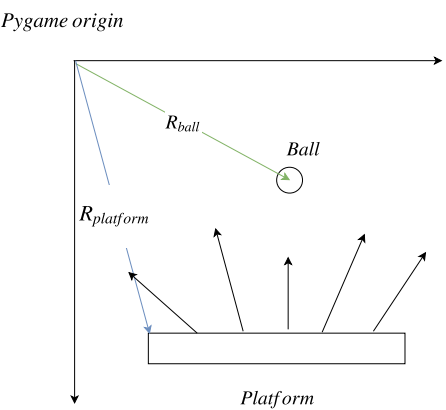
\includegraphics[width=0.60\textwidth]{platform.png}
}
\caption{Hvordan ballen skal sprette i forhold til hvor på platformen den treffer.}
\label{newcoord}
\end{figure}

I pygame vil koordinatsystemet ha origo i venstre hjørnet slik som i figur(\ref{newcoord}). Herfra trekkes det vektor ned til sentrum av platformen for å translatere origo dit. Deretter lages det en liste med verdier fra en cosinus funksjon i intervallet $\pi$ til 0. Da vil verdier på platformen være -1 til 1, fordeler man dette ut på platformen slik at origo(midten av platformen) vil ha verdi 0($\cos(90\degree) = 0$) kan man sette hastigheten i x-retning til ballen til disse verdiene. Da vil ballen ha negativ hastighet i x-retning hvis den treffer på venstre siden av platformen og en positiv hastighet hvis den treffer på høyre siden(av origo). Verdien vil bli større i x retning etter hvor lengre ut mot sidene ball treffer slik at ballen får en brattere vinkel mot sidene.
Platformen skal også kunne styres av spilleren ved hjelp av piltastene. Hastigheten på platformen må følge FPS(frames per second) som er låst til 60(styres av pygame clock funksjon) slik at den ikke går kjappere hvis man spiller på en kraftigere pc.\\

\emph{move}: Flytter posisjonen til ballen basert på x og y hastighetskomponentene, i dette tilfelle vil det kun være bevegelse i x-retning. Det spesielle her er at platformen kontrolleres ved hjelp av tastaturet så her brukes \emph{pygame.key.get\_pressed()} metoden for å hente ut tastetrykk. Her blir time\_passed\_seconds sendt inn i metoden for å skalere ned farten slik at den er konstant uavhengig av FPS.\\\\

\emph{def draw(self)}: Tegnefunksjonen som vil tegne platformen ut på spillvinduet.


\subsection{Ball}

Ballen skal sprette av både platformen og blokkene. Ved å gange hastigheten med -1 vil ballen reflektere ut med samme vinkel uten demping.
Ballen skal ha en maks fart uansett hvor stor komponent det er i x eller y, så her er det brukt enhetsvektor med en skalering.
\begin{equation}
    \vect{V}_{ball} = \frac{\vect{v}_{ball}}{||\vect{v}_{ball}||}\alpha
\end{equation}
,der $\alpha$ er en skalar for hva farten skal være slik at,
\begin{equation}
     ||\vect{V}_{ball}|| = \alpha, \, \forall\,t
\end{equation}
Dette vil gi oss posisjonen gitt ved,
\begin{equation}
    (x,y) = \vect{V}_{ball}t\footnote{I programmet vil ikke dette være tid direkte, men ved FPS. Hvis man har 60 FPS vil denne operasjonen skje 60 ganger per sekund. Her vil vi derfor legge inn en skalarverdi fra pygame sin clock funksjon som skalerer farten slik at den holder seg konstant for all FPS.}
\end{equation}

Ballen skal også knuse blokker når den treffer dem og sprette vekk igjen, men dette vil bli kontrollert av bricks objektene i denne oppgaven.

Disse metodene vil bli brukt i spill-løkken som forklart i seksjon(\ref{Gameloop}).\\\\

\emph{move}: Flytter posisjonen til ballen basert på x og y hastighetskomponentene. Her blir time\_passed\_seconds sendt inn i metoden for å skalere ned farten slik at den er konstant uavhengig av FPS.\\\\

\emph{check\_wall\_collisions}: Sjekker om ballen treffer veggene, her brukes størrelsen på spillvinduet og radiusen til ballen for å sjekke for kollisjon,i figur(\ref{ball}) under vises dette.\\\\
\begin{figure}[H]
\center{
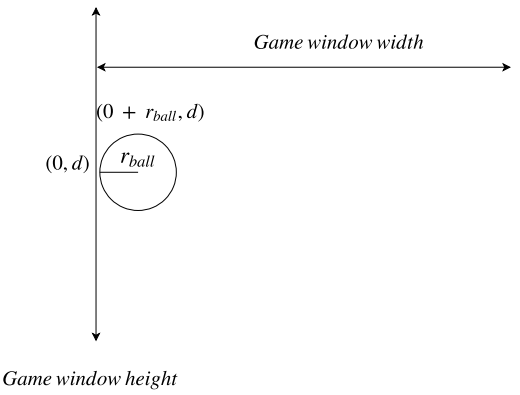
\includegraphics[width=0.65\textwidth]{ball_sketch.png}
}
\caption{Siden origo til ballen ligger i sentrum må det testes for når ballens posisjon og radius kommer utafor skjermen.}
\label{ball}
\end{figure}


\emph{check\_platform\_collision(self, platform)}: Her sjekkes det om ballen treffer platformen, her skal noe av det samme skje som med veggene men at ballen også skal bli gitt en x-hastighet som er større hvor lengre ut på sidene ballen treffer på platformen. Dette vil forårsake at ballen blir reflektert med en vinkel. Her blir platform objektet tatt inn som argument og deretter brukes posisjonen til platformen får å finne ut om den kolliderer.\\\\

\emph{def draw(self)}: Til slutt er det tegnefunksjonen som vil tegne ballen ut på spillvinduet, dette vil være felles for alle objektene.




\subsection{Bricks}

Brikkene skal bli borte når de blir truffet av ballen. Ballen skal også sprette vekk igjen når den treffer brikkene. Brikkene plasseres ved siden av hverandre i en gitt distanse og med N rader, dette blir styrt ved en \textcolor{purple}{global} variabel i konfigurasjonsfilen. Brikkene har en \emph{health}(helse) attributt som bestemmer hvor mange ganger ballen må treffe før den blir ødelagt(I denne oppgaven blir brikkene gitt 1 helse). Ved å lage en sammenheng mellom farge og helse kan man sette forskjellige farger etter hvor mye helse en brikke har.\\
\emph{hit\_detection}: Denne metoden tar inn Ball objektet for å finne posisjonen til ballen og en brick for å få posisjonen til brikken. Dermed sjekkes det om ballen er innenfor brikken høyde og bredde. Hvis dette er sant returneres True. Legg også merke til at denne metoden er en @staticmethod, dette betyr at den kan bli kalt på via klassen.\\\\

\emph{update\_bricks(Ball)}: Sjekker om ballen har truffet en brikke(ved hjelp av \emph{hit\_detection} metoden) og fjerner så et liv fra brikken. Hvis livet til brikken er under 0 vil brikken bli slettet fra en brick\_list som er en klasseliste som holder på alle brikkene som er ute i spillet. Hvis en brille blir fjernet fra denne listen vil den ikke bli tegnet i spill vinduet.\\\\


\emph{initiate\_bricks(rows)}: Denne metoden blir initialisert når programmet starter. Denne laster inn brikker gitt ved variablen \textcolor{purple}{NUMBER\_OF\_BLOCK\_HORIZONTAL} og rows som angir hvor mange rader med brikker det skal være.\\

I denne koden kan man se hvordan en dobbel for-løkke blir brukt til å lage rad og kolonner med brikker. Her blir et nytt objekt av typen \emph{Bricks} lagt til i klasse listen \emph{bricks\_list} og der \textcolor{purple}{globale} variablene fra konfigurasjonsfilen hjelper til med å lage distanse imellom brikkene.\\\\

\emph{def draw(self)}: Tegnefunksjonen som vil tegne brikkene ut på spillvinduet.




\subsection{Konfigurasjonsfilen}

Konfigurasjonsfilen(\textcolor{blue}{config.py}) inneholder alle \textcolor{purple}{globale} variabler. Denne blir brukt slik at man unngår \emph{magic numbers}(tall i koden det er vanskelig å tolke hva gjør) og at man enkelt kan endre på innstillingene i programmet.



\section{Implementasjon}
\subsection{Kodespråk}
Koden er skrevet i Python versjon 3.\footnote{https://www.python.org/}\\
\subsection{Operativsystem og enheter}
OS: Windows 10\\
Systemtype: 64-bit OS, x64-basert prosessor
Skjermkort: NVIDIA Geforce 920MX\\
CPU: Intel(R) Core(TM) i5-7200U CPU @ 2.50GHz\\
RAM: 4GB
\subsection{Moduler}
Pygame \footnote{https://www.pygame.org/wiki/GettingStarted} Version: 1.9.4\\
Nympy \footnote{http://www.numpy.org/} Version: 1.14.5\\


% Dette prosjektet er implementert i Python\footnote{https://www.python.org/} versjon 3.6 eller større og Pygame modul\footnote{https://www.pygame.org/wiki/GettingStarted} som blir brukt til å tegne til skjermen. I dokumentasjonen til Pygame står det også om hvordan man initialiserer pygame vinduet som er nyttig for å komme igang.

\section{Diskusjon}

Første gang denne oppgaven ble gjennomført var oppgaven løst ved å kun oppfylle kravene. Da spillet var ferdig ble menyer, toppliste, forskjellige spill nivåer og musikk implementert. Dette førte til at koden ble veldig ustrukturert og vanskelig å navigere fordi det ikke var planlagt når oppgaven ble påbegynt. Derfor ble oppgaven løst på nytt med bedre kodestruktur. Det å planlegge alt først før man gjennomfører viser å være viktig for at kodestrukturen skal være så fin som mulig. I oppgaven ble det også brukt \emph{@staticmethod} et $"$problem$"$ i dette tilfelle er at disse gjorde en god del krevende arbeid som dobbel for-løkke osv, og er ment for å kun kjøre fra et kall til klassen. Men staticmethod tillater også instanser fra klassen å kalle på disse metodene, slik at hvis man er $"$uheldig$"$ og kaller på disse inne i løkkene som jobber med metodene til objektene vil det sakte ned pc'en betraktelig. Det er også viktig å merke seg er at koordinatsystemet i pygame er i tredje kvadrant med snudd y-akse som vist i figur(\ref{akse}) under.

\begin{figure}[H]
\center{
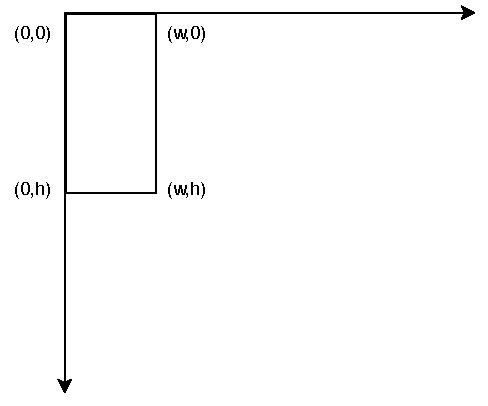
\includegraphics[width=0.60\textwidth]{akse.pdf}
}
\caption{En rektangel tegnet i posisjon (0,0) med bredd w og høyde h.}
\label{akse}
\end{figure}

Hvordan ballen samhandler med platformen kunne hvert gjort på mange måter. I dette oppgaven gjorde vi det veldig enkelt ved å $"$strekke$"$ en sirkel ut i en en-dimensjonell array som inneholder trigonometriske verdiene slik at $\cost(\pi)$ er på første indeks og 0 er på siste.
\begin{lstlisting}
anglelist = [\cost(\pi),\cost(..), .....,\cost(0)]
\end{lstlisting}
Disse ble fordelt utover platform bredden slik at $\frac{\pi}{2}$ ligger ca i midten.
Disse verdiene blir gitt til x-hastigheten til ballen etter hvor på platformen den treffer. Plasseringen til ballen på platformen angir hvilken indeks verdi som blir gitt til ballens x-hastighet og derfor vil dette da bli en tilnærming da indeksene er diskré verdier. Et eksempel er hvis ballen treffer på plass 0.12 vil denne bli rundet ned til indeks 0 som er $cos(\pi) = -1$.


\subsection{Evaluasjon}

Implementerte en FPS(Frames per second) funksjon for å se hvor optimalisert koden er. I figur(\ref{FPS}) ser man resultatet av FPS'en. Den ser ut til å flukturere rundt 60 FPS som har blitt satt ved å pygames clock funksjon. FPS'en vil variere etter hvor kraftig pc man har, men den skal være låst til rundt 60.



\begin{figure}[h!]
\center{
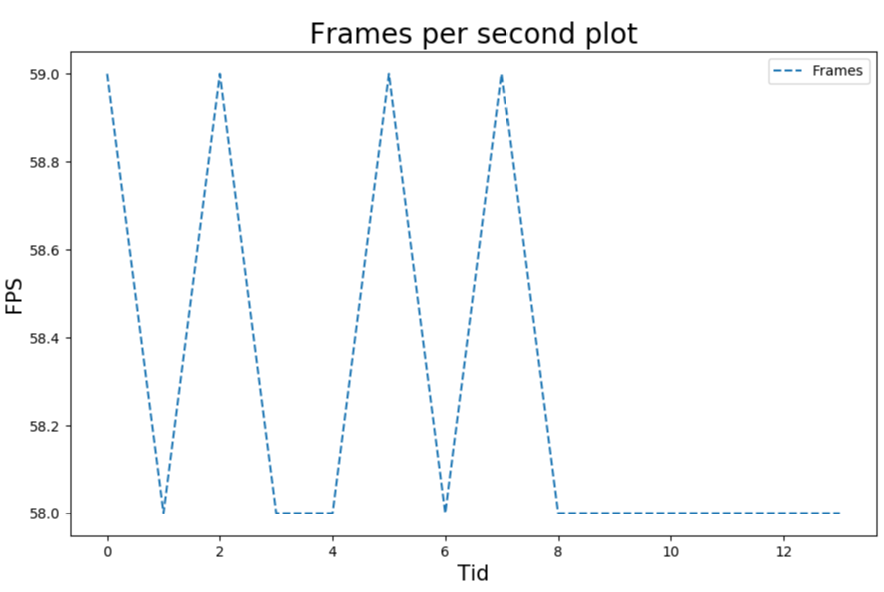
\includegraphics[width=0.85\textwidth]{FPS.png}
}
\caption{Frames per second(FPS) under testing av koden, her er x-aksen i sekunder.}
\label{FPS}
\end{figure}

\section{Konklusjon}

I denne oppgaven ble en klone av spillet \emph{Breakout} laget ved bruk av python, Pygame og objektorientert design. Her vises det at det kan enkelt bli gjennomført strukturert. Et problem som oppsto er det at koden blir ustrukturert hvis man implementerer flere funksjoner til koden som man ikke hadde planer om å ta med fra starten av uten å måtte veldig mye tid på å restrukturere koden.










\newpage
\appendix
%Her starter man appendiksene. Det er ekstraseksjoner som ikke er essensielle for rapporten, men kan være nyttige.

\section{Appendix}
%Legg ved supplementer informasjon
%Script brukt til viktig dataanalyse
%Detaljert utledning av nye/viktige ligninger
%Kalibreringsmålinger






% \section{Referanser}

% \nocite{math}
% \nocite{wiki}
% \nocite{cornel}

% \nocite{wikicoef}



\bibliographystyle{plainnat}
\bibliography{bibl}



%Bibliografien kommer til slutt.
\end{document}
